\emph{Transformation and Performance Consultants} (\entreprise) est un cabinet \og multi spécialiste \fg hybride et indépendant qui intervient dans la mise en place de programmes de transformation auprès de grands groupes.
L'entreprise a été créée en 2007 par Benoit \textsc{Ranini} et Guy \textsc{LETURCQ}.

Le cabinet apporte son expertise et son savoir-faire dans la mise en place de modèles opérationnels pour dynamiser la performance des entreprises et leur permettre de créer toujours plus de valeur ajoutée. Il est détenu à 100\% par les associés.

\entreprise est en pleine croissance avec 50 millions d’euros de chiffre d’affaires en 2017, 60 millions en 2018, 85 millions en 2019 et une prévision de 100 millions pour 2020.
Plusieurs cabinets dans le monde ont été ouverts, 23 nationalités y sont réunies, et plus d'une quinzaine de langues sont parlées entre tous les collaborateurs. 

Le cabinet se veut innovant, et a ainsi investi dans plusieurs incubateurs de start-ups en France comme le Gate 31, l'IoT Valley ou le T-Hub.

Les principaux secteurs de \entreprise sont le bancaire (Société Générale, \textsc{BNP} Paribas, etc.), l'assurance et protection sociale (\textsc{AXA}, \textsc{AG2R}, etc.), la santé et le secteur public (Agirc-Arrco, marine nationale), des mobilités (\textsc{SNCF}, \textsc{RATP}, Airbus) et enfin l'industrie et service (\textsc{EDF}, Total, \textsc{LVMH}, Carrefour, etc.).
L'entreprise est également découpée en offres
\footnote{Le sous-secteur mobilités est devenu un secteur depuis l'illustration}.

\begin{figure}[H]
    \centering
    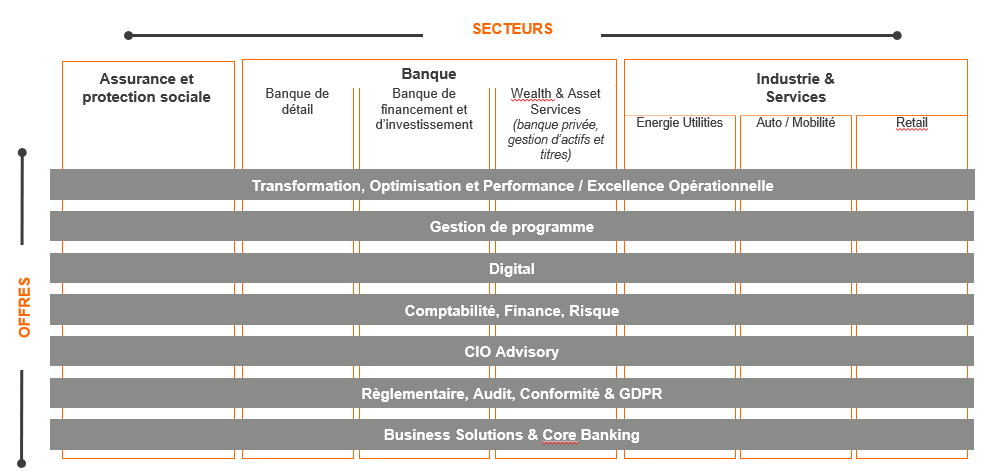
\includegraphics[width=1\linewidth]{img/tnp_secteurs_offres.png}
    \caption{Secteurs et offres de \entreprise{}  }
\end{figure}

Le service \df dans lequel je travaille, et qui a réalisé la mission \emph{bouclage de production}, se trouve dans l'offre \emph{Digital \& Solutions}.

Encore une fois, l'offre est divisée en sous-offres ayant chacune leurs spécialités.

\begin{figure}[H]
    \centering
    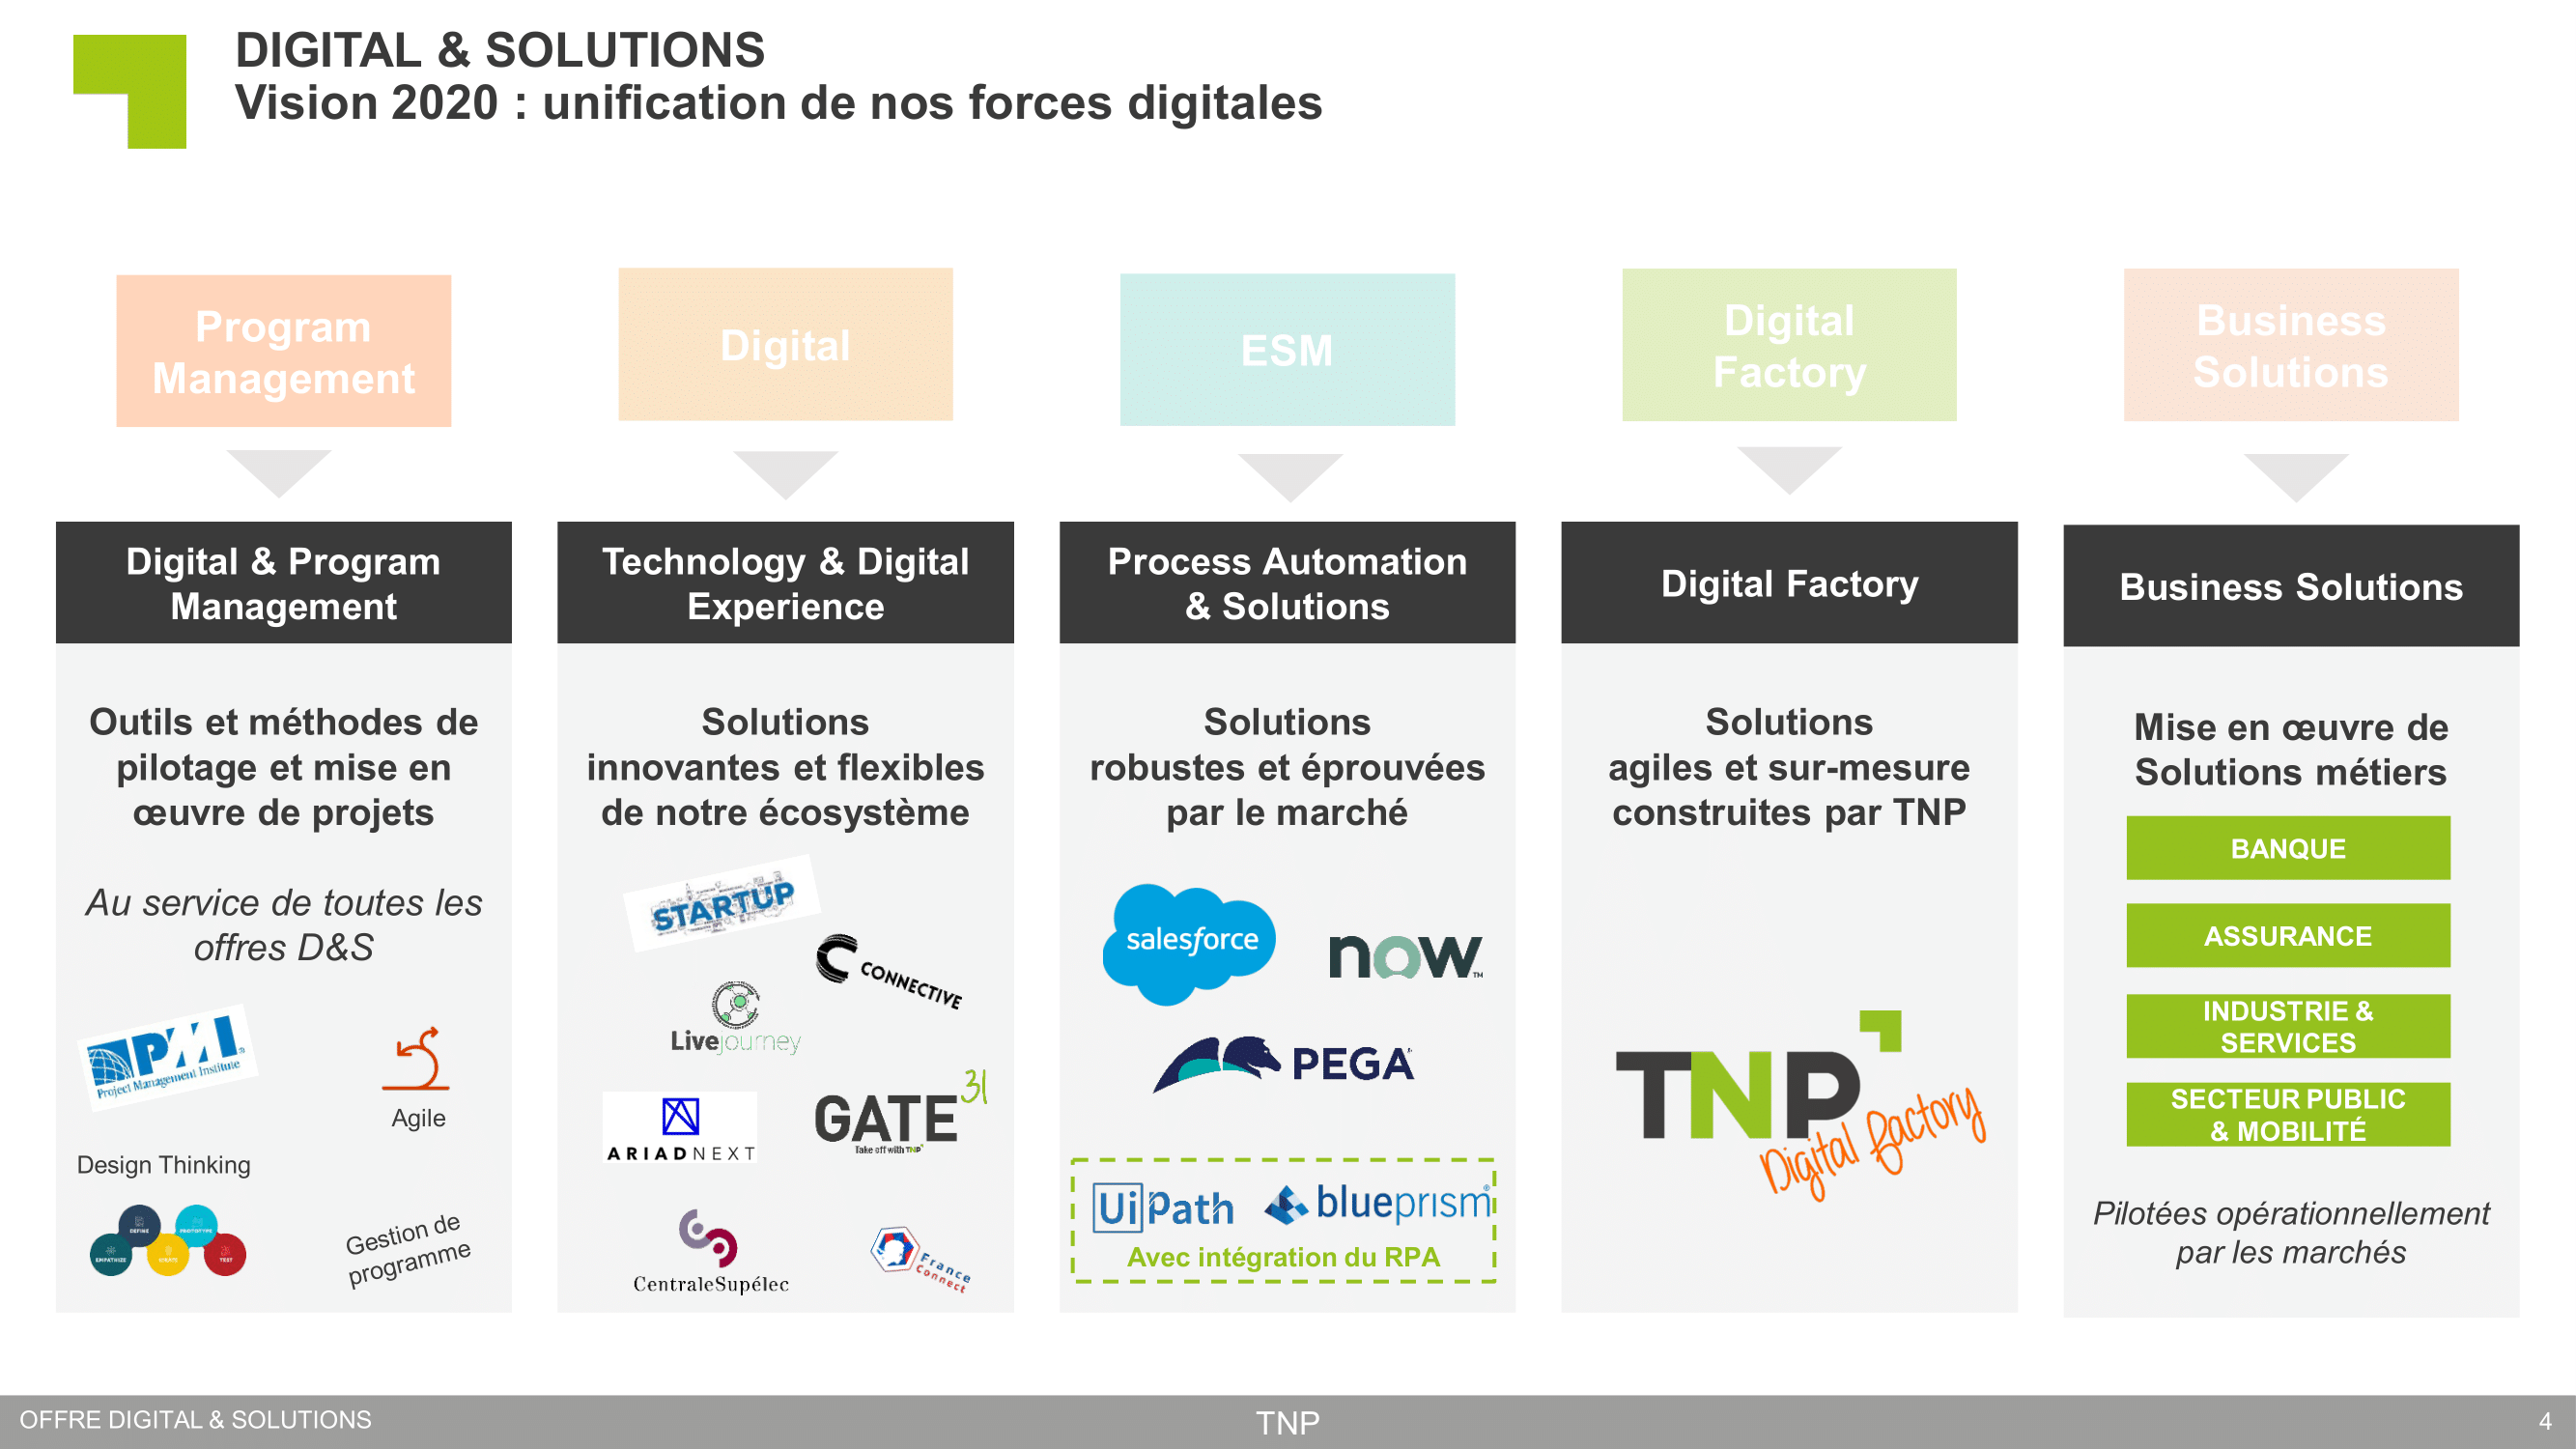
\includegraphics[width=1\linewidth]{img/Offre digital and solutions TNP_20200131-05.png}
    \caption{Les différentes sous-offres au sein de Digital \& Solutions}
\end{figure}

\begin{figure}[H]
    \centering
    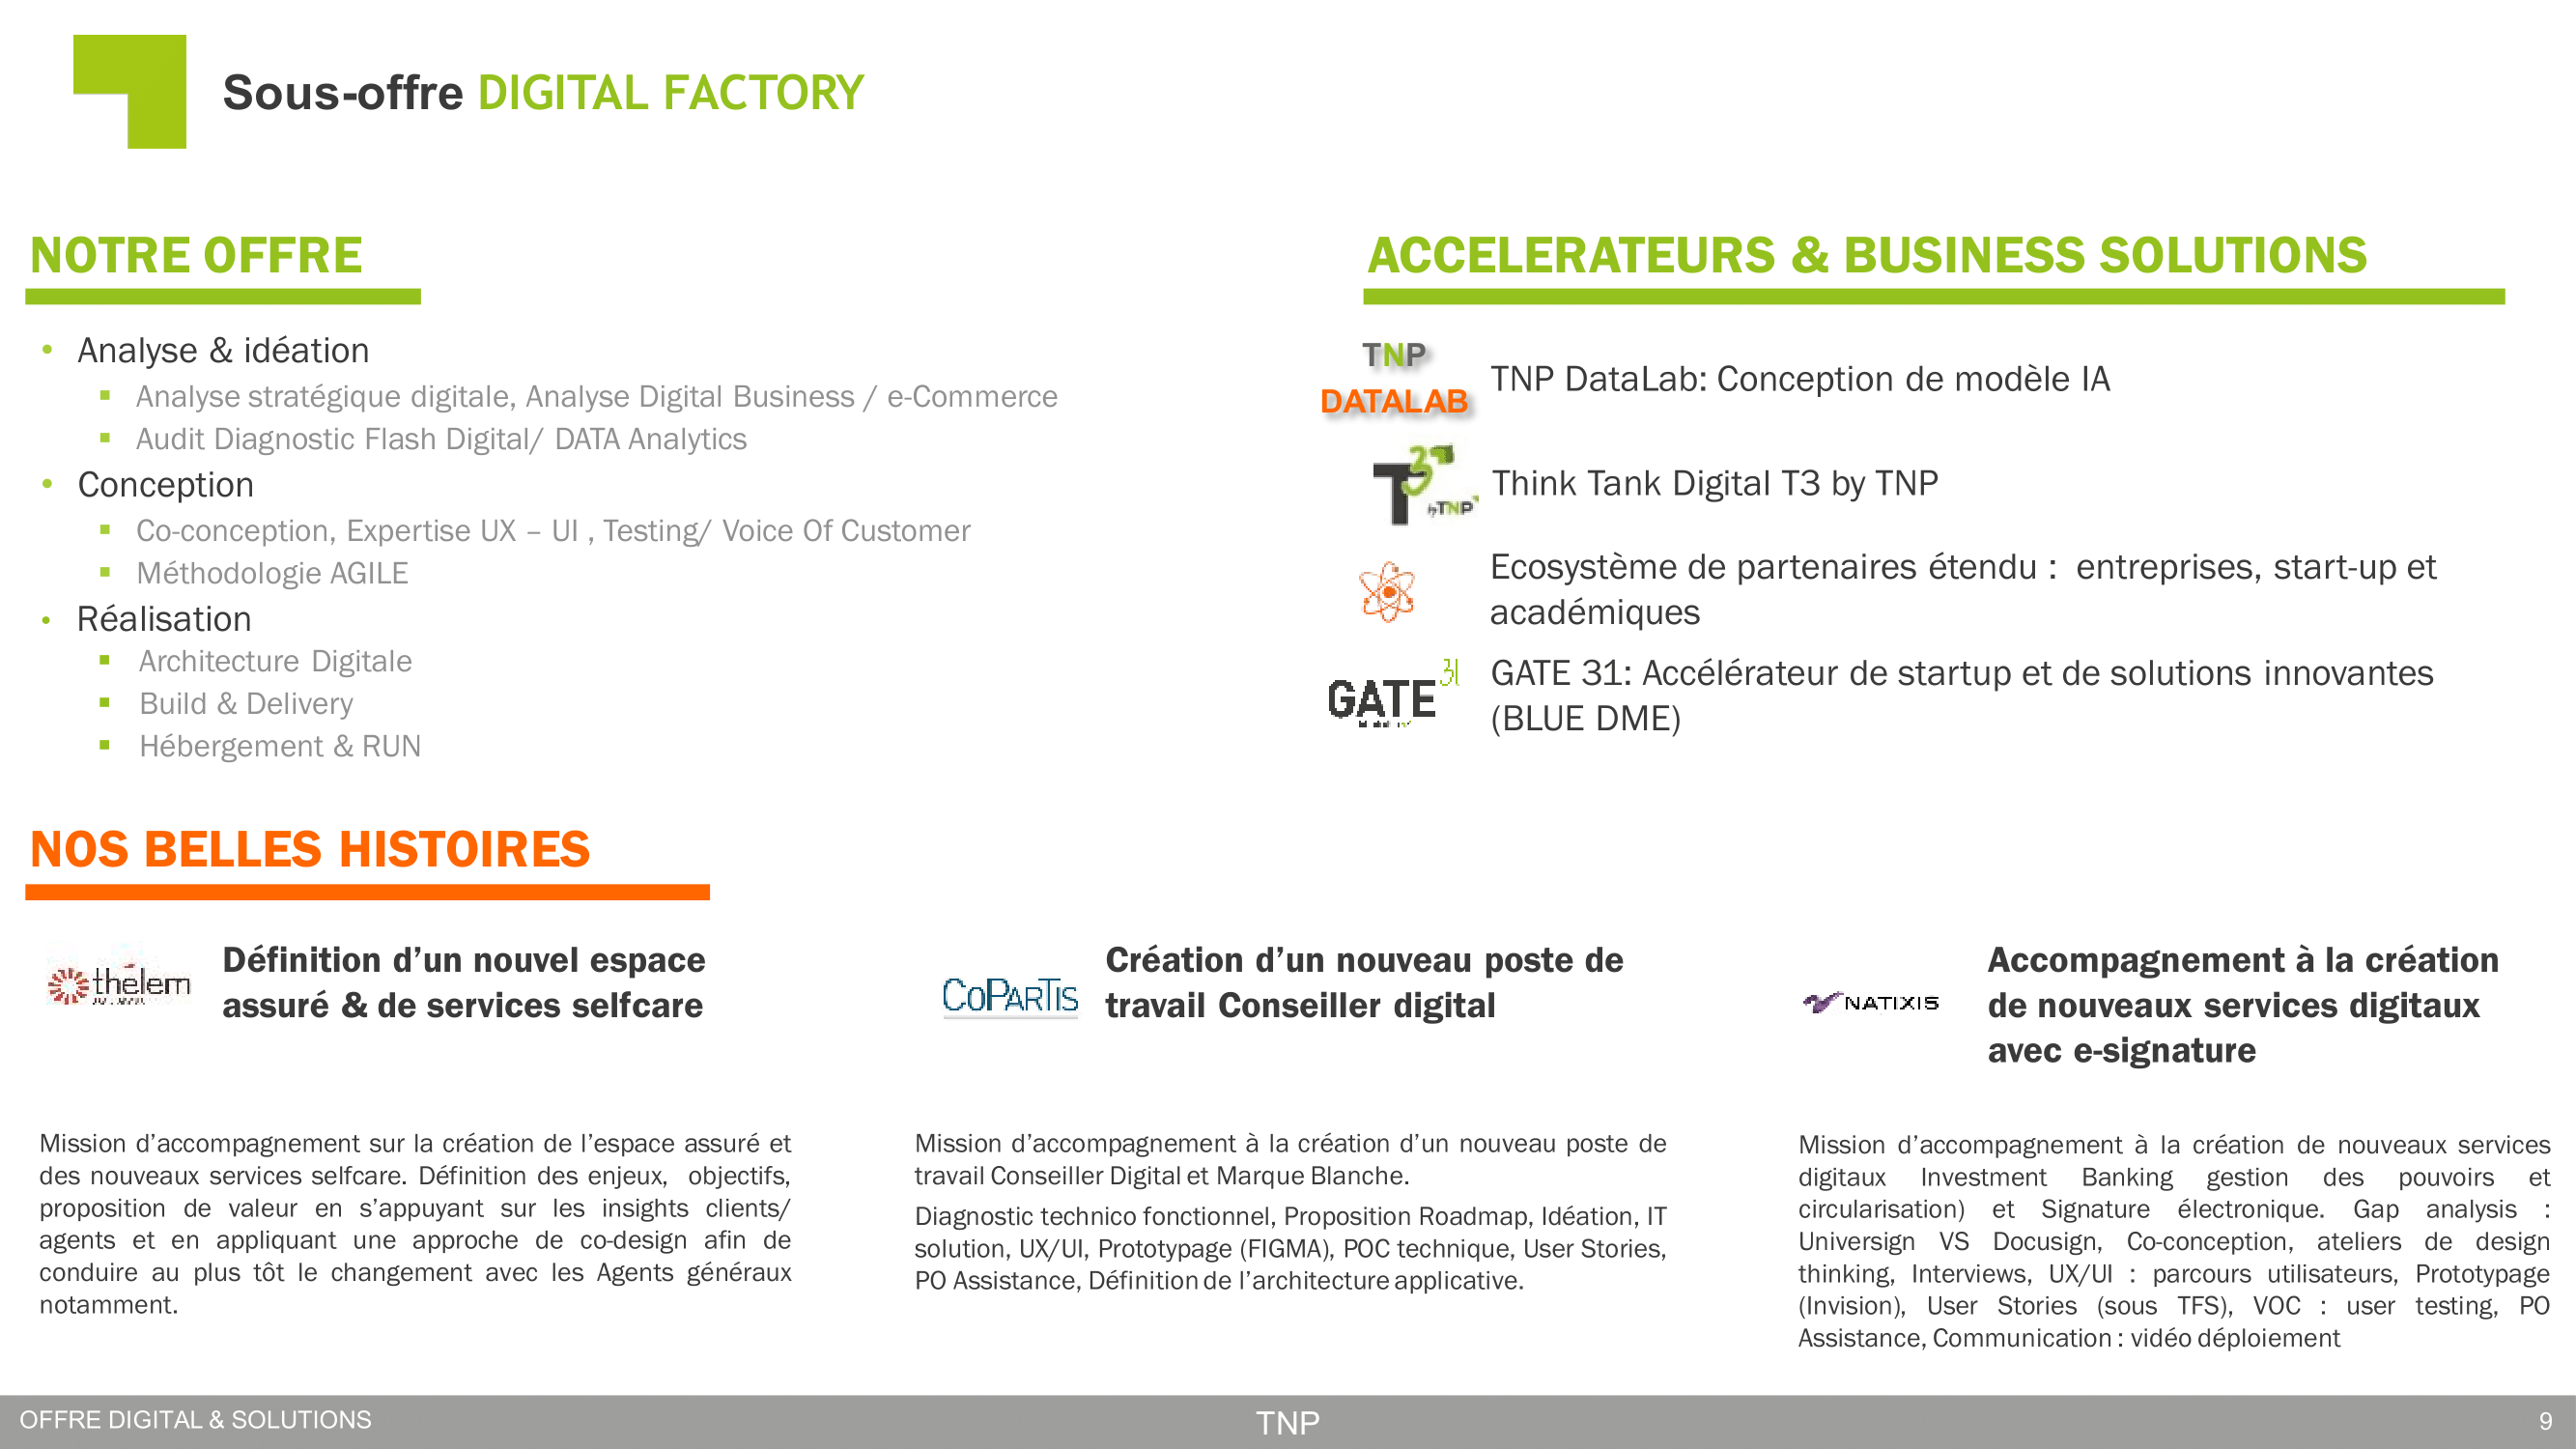
\includegraphics[width=1\linewidth]{img/Offre digital and solutions TNP_20200131-10.png}
    \caption{La sous-offre Digital Factory}
\end{figure}

Jusqu'à présent \entreprise, via son offre Digital \& Solutions, ne faisait qu'accompagner les entreprises dans leur transformation numérique. La \df permet au cabinet de proposer des solutions créées en interne chez \entreprise, ou bien de concevoir pour le client le produit répondant à ses besoins.

Ainsi, la \df permet de compléter l'offre du cabinet, en allant du conseil jusqu'à la réalisation concrète.\\
L'offre a été créée en mai 2019, et est pour le moment constituée de deux équipes: la data science et le développement web et mobile.